\section{Сигнальные процессы}

\subsection{Тёмный фотон}

Одним из популярных гипотетических механизмов описания связи \acrshort{dm}
с физикой СМ является расширение групп симметрии 
лагранжиана СМ путем добавления абелевой калибровочной группы $U_D(1)$, 
действующей в секторе темной материи~\cite{holdom} и кинетически смешанной 
с абелевой электромагнитной группой $U_{\textrm em}(1)$:
\begin{equation}
\label{LCM_A}
    \mathcal{L}_{SM+A'} = \mathcal{L}_{SM} + \epsilon \, F^{\mu\nu} F'_{\mu \nu}
        - \frac{1}{4} F'^{\mu\nu} F'_{\mu\nu} + \frac{m_{A'}^2}{2} m_{A'}^2 A'^{\mu}A'_{\mu},
\end{equation}
где
% совет: "должна быть полная расшифровка всех величин"
$\mathcal{L}_{SM}$ --- лагранжиан \acrshort{sm}, 
$A'_{\mu}$ и $m_{A'}$ --- полевой оператор и масса тёмного фотона, 
который является массивным векторным бозоном, 
$F_{\mu \nu}$ и $F'_{\mu \nu}$ --- тензоры напряженности 
электромагнитного поля (фотона) и поля тёмного фотона, соответственно,
$\epsilon_Y$ --- константа взаимодействия  
электромагнитного поля и поля темного бозона. 

% NOTE  ГОСТ Р2 . 105 - 2019:
%       "Пояснения символов и числовых коэффициентов, входящих в формулу, если
%       они не пояснены ранее в тексте, должны быть приведены непосредственно
%       под формулой. Пояснения каждого символа следует давать с новой строки
%       в той последовательности, в которой символы приведе
%       ны в формуле. Первая строка пояснения должна начинаться со слова
%       «где» без двоеточия после него."
% при этом:
% NOTE  В ГОСТах, регламентирующих оформление научной и технической документации
%       (например, ГОСТ 7.32-2001 и ГОСТ 2.105-95, знаки пунктуации в конце
%       отдельно стоящих формул _указываются_)

Далее в лагранжиане~(\ref{LCM_A}) вводится взаимодействие тёмного 
фотона с фермионами \acrshort{sm} $\psi$:
\begin{equation}
\label{L_Apsi}
    \mathcal{L}_{A\bar\psi\psi} = \epsilon \, A'_\mu  
    \bar\psi \gamma^\mu Q_\psi \psi 
\end{equation}
где $Q_\psi$ --- электрический заряд СМ фермиона (заряженный лептон или кварк), 
производя сдвиг электромагнитного поля 
$A_\mu(x) \to A_\mu(x) + \epsilon \, A'_\mu(x)$, который также устраняет 
смешивание наблюдаемого и темного фотона, т.е. член 
$\epsilon \, F^{\mu\nu} F'_{\mu \nu}$.

Экспериментальное наблюдение взаимодействия описанного
лагранжианом~\eqref{LCM_A} может быть произведено, например,
в реакции фотообразования при рассеянии
электрона на тяжёлом ядре, изображённой на рисунке \ref{fig:aprime-production}.
Интегрирование матрицы рассеяния позволяет получить приблизительные
количественные оценки для постановки таких экспериментов на
ускорителях обеспечивающих энергию лептонов порядка
нескольких сотен ГэВ.

\subsection{Лёгкие аксион-подобные частицы}

Наряду с тёмным фотоном в литературе существует другой хорошо мотивированный 
тип частиц новой физики --
аксион-подобные частицы $a$~(\emph{axion-like particles} --ALPs)~\cite{Dobrich2016}), 
предложеных Пессей-Куинн~\cite{Peccei:1977hh}, Вайнбергом~\cite{Weinberg:1977ma} 
и Вильчеком~\cite{Wilczek:1977pj} 50 лет назад. 

%\begin{wrapfigure}{r}{0.35\textwidth}
\begin{figure}
    \centering
    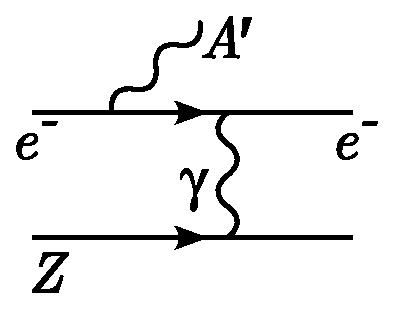
\includegraphics[width=.55\linewidth]{images/illustrative/aprime-photoprod.eps}
    \caption{Фоторождение $A'$ на ядре $Z$}
    \label{fig:aprime-production}
\end{figure}
%\end{wrapfigure}

Постулируя, что $a$ является псевдоскалярной частицей, можно построить 
феноменологический лагранжиан, описывающий его свободное движение и взаимодействие 
с электромагнитным полем 
\begin{equation}
    \mathcal{L}_{F+a} = - \frac{1}{4} g_{a \gamma \gamma} a F_{\mu \nu} \tilde F_{\mu \nu}
        + \frac{1}{2} (\partial_{\mu} a)^2 - \frac{1}{2} m^2_a a^2,
\end{equation}
где $\tilde{F}_{\mu \nu} = \frac{1}{2} \epsilon_{\mu \nu \lambda \rho} F^{\lambda \rho}$ --- дуальный тензор электромагнитного поля,
$g_{a \gamma \gamma}$ -- константа связи, и $m_a$ -- масса ALP частицы.

Эксперимент по поиску $a$ подразумевает постановку схожую с экспериментом
по поиску $A'$. Диаграмма реакций приведена на рисунке~\ref{fig:axion-photo}.

\begin{figure}[ht]
    \centering
    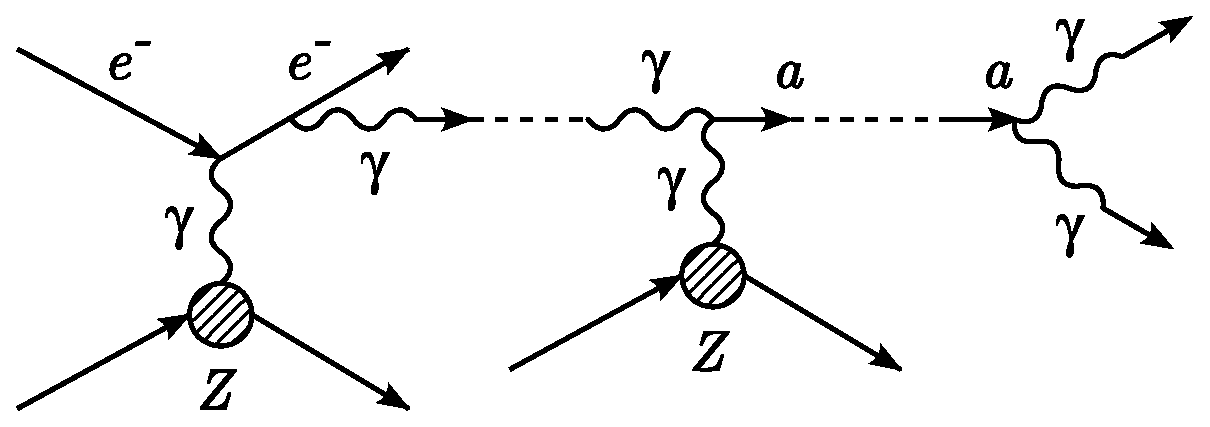
\includegraphics[width=0.75\linewidth]{images/illustrative/ALPs-photoprod-ours.eps}
    \caption{Фоторождение и распад аксион-подобной частицы (ALP).}
    \label{fig:axion-photo}
\end{figure}